\documentclass{article}
\title{Ciclo de vida de una empresa}
\author{David Gabriel Corzo Mcmath}
\date{2020-Jan-18 13:46:39}
%%%%%%%%%%%%%%%%%%%%%%%%%%%%%%%%%%%%%%%%%%%%%%%%%%%%%%%%%%%%%%%%%%%%%%%%%%%%%%%%%%%%%%%%%%%%%%%%%%%%%%%%%%%%%%%%%%%%%%%%%%%%%%%%%%%%%%%%%%%%%%%
\usepackage[margin = 1in]{geometry}
\usepackage{graphicx}
\usepackage{fontenc}
\usepackage{pdfpages}
\usepackage[spanish]{babel}
\usepackage{amsmath}
\usepackage{amsthm}
\usepackage[utf8]{inputenc}
\usepackage{enumitem}
\usepackage{mathtools}
\usepackage{import}
\usepackage{xifthen}
\usepackage{pdfpages}
\usepackage{transparent}
\usepackage{color}
\usepackage{fancyhdr}
\usepackage{lipsum}
\usepackage{sectsty}
\usepackage{titlesec}
\usepackage{calc}
\usepackage{lmodern}
\usepackage{xpatch}
\usepackage{blindtext}
\usepackage{bookmark}
\usepackage{fancyhdr}
\usepackage{xcolor}
\usepackage{tikz}
\usepackage{blindtext}
\usepackage{hyperref}
\usepackage{listing}
\usepackage{spverbatim}
\usepackage{fancyvrb}
\usepackage{fvextra}
\usepackage{amssymb}
\usepackage{pifont}
\usepackage{longtable}
%%%%%%%%%%%%%%%%%%%%%%%%%%%%%%%%%%%%%%%%%%%%%%%%%%%%%%%%%%%%%%%%%%%%%%%%%%%%%%%%%%%%%%%%%%%%%%%%%%%%%%%%%%%%%%%%%%%%%%%%%%%%%%%%%%%%%%%%%%%%%%%
\begin{document}
\maketitle


\section{Lanzamiento y crecimiento}
A partir del año 1999 se introdujo al mercado un nuevo celular, el BlackBerry. Hoy en día se sabe que ya nadie usa el blackberry, pero \textbf{Nos preguntamos:} ¿porqué?... 
Empecemos desde el principio, el lanzamiento de BlackBerry en Guatemala se dio un crecimiento exponencial, en asunto de unos cuantos años todos tenían un Blackberry. Cuando los blackberryies estaban de moda estaban atendiendo una necesidad muy puntual, la gente veía valor poder comunicarse por medio de un mensaje y dejar de pagar altas tarifas telefónicas llamando por teléfono, entonces la idea de poderse comunicar por un dispositivo pequeño y versátil era algo innovador.

\subsection{Competencia de Apple}
A finales de la primera década del siglo 21 se introduce en 2007 el primer iPhone, respondiendo a una tendencia muu importante que los usuarios tenían, muchos veían cosas innovadoras con el iPhone. Introducen el teclado touch y una rápidez de procesamiento que anteriormente el mercado desconocía.


\section{Ciclo de vida}
\begin{enumerate}
    \item Incio y crecimiento:
        \begin{itemize}
            \item Cuando BlackBerry empezó se introdujo un nuevo innovador producto que se lanzó a la sima a lo largo de tan sólo algunos años.
        \end{itemize} 
    \item Crecimiento exponencial:
        \begin{itemize}
            \item Posteriormente se empezó a expandir a lo largo del mercado mundial llegando a ser en un momento el celular más popular del momento.
        \end{itemize}
    
    \item Madurez:
        \begin{itemize}
            \item Cuando Blackberry madura surgen bastantes competidores muy buenos que tenían mucho más energía que Blackberry y que rápidamente tomaron el mercado, en específico iPhone en 2007, hoy en día Apple es la empresa más grande llegando a estar valorada cerca del trillón de dólares.
            \item Esto destruyó a blackberry y a pesar de sus diversos intentos de querer reincorporarse al mercado no se pudo por lo cual esta época hizo que Blackberry decayera hasta llegar al nivel obsoleto.
        \end{itemize}
    
    \item Terminación: 
        \begin{itemize}
            \item Hoy en día blackberry no es relevante en el mercado en el cual un día fue tan grande, se trata de tomar una lección a lo que pasó, suponemos que este fenómeno de destrucción creativa surgió por que Blackberry se acomodó en todo su éxito y esto en suma provocó su decadencia.
        \end{itemize}
\end{enumerate}

\section{Estado actual}
Hoy en día Blackberry se ha quedado en un estado obsoleto al menos en el mercado que solía manejar con tanta influencia.

\section{Imagenes}
\begin{figure}[htbp]
    \centering
    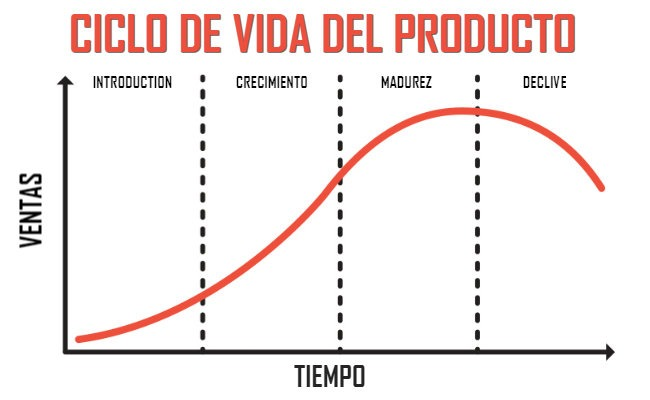
\includegraphics[width=8cm]{ciclo-de-vida-del-producto.jpg}
    \caption{Apreciamos cómo se desempeña una empresa a lo largo de su vida, en este caso una terminación en decadenecia.}
    \label{}
\end{figure} 

\end{document}